\subsection{External Interface Requirements}
\subsubsection{User Interfaces}
The platform will have a web interface accessible via browser from both students and educators. 
Now, some mockups of the main pages of the platform will be presented, organized by functionality.

\begin{enumerate}[label=\textbf{F\arabic*)}]
    \item \textbf{Signup and Login}\\
    The signup page asks to the unregistered user to provide some personal information like name, surname, email address and password. Moreover, the user has to specify if he is a student or an educator by flagging the corresponding checkbox. In case he is a student, he is also asked to provide his GitHub's username. Alternatively, users can choose to sign up using third party services like Google or GitHub.\\
    \begin{figure}[H]
        \centering
        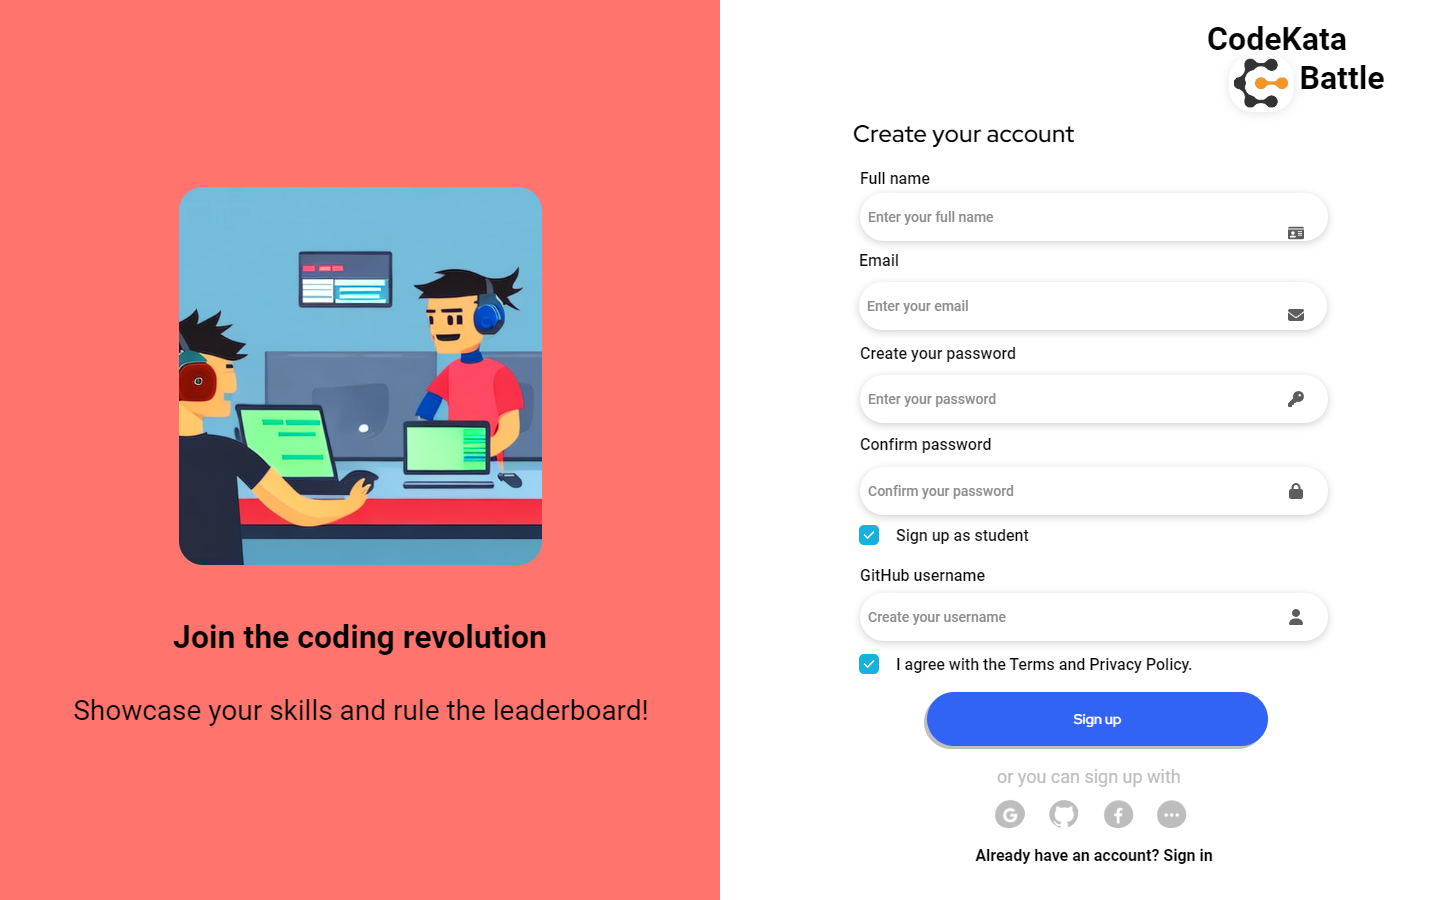
\includegraphics[width=0.8\textwidth]{Mockups/1_signup.png}
        \caption{Signup page}
    \end{figure}
    The login page asks to the registered user to provide his email address and password. Alternatively, users can choose to login using third party services like Google or GitHub.\\
    \begin{figure}[H]
        \centering
        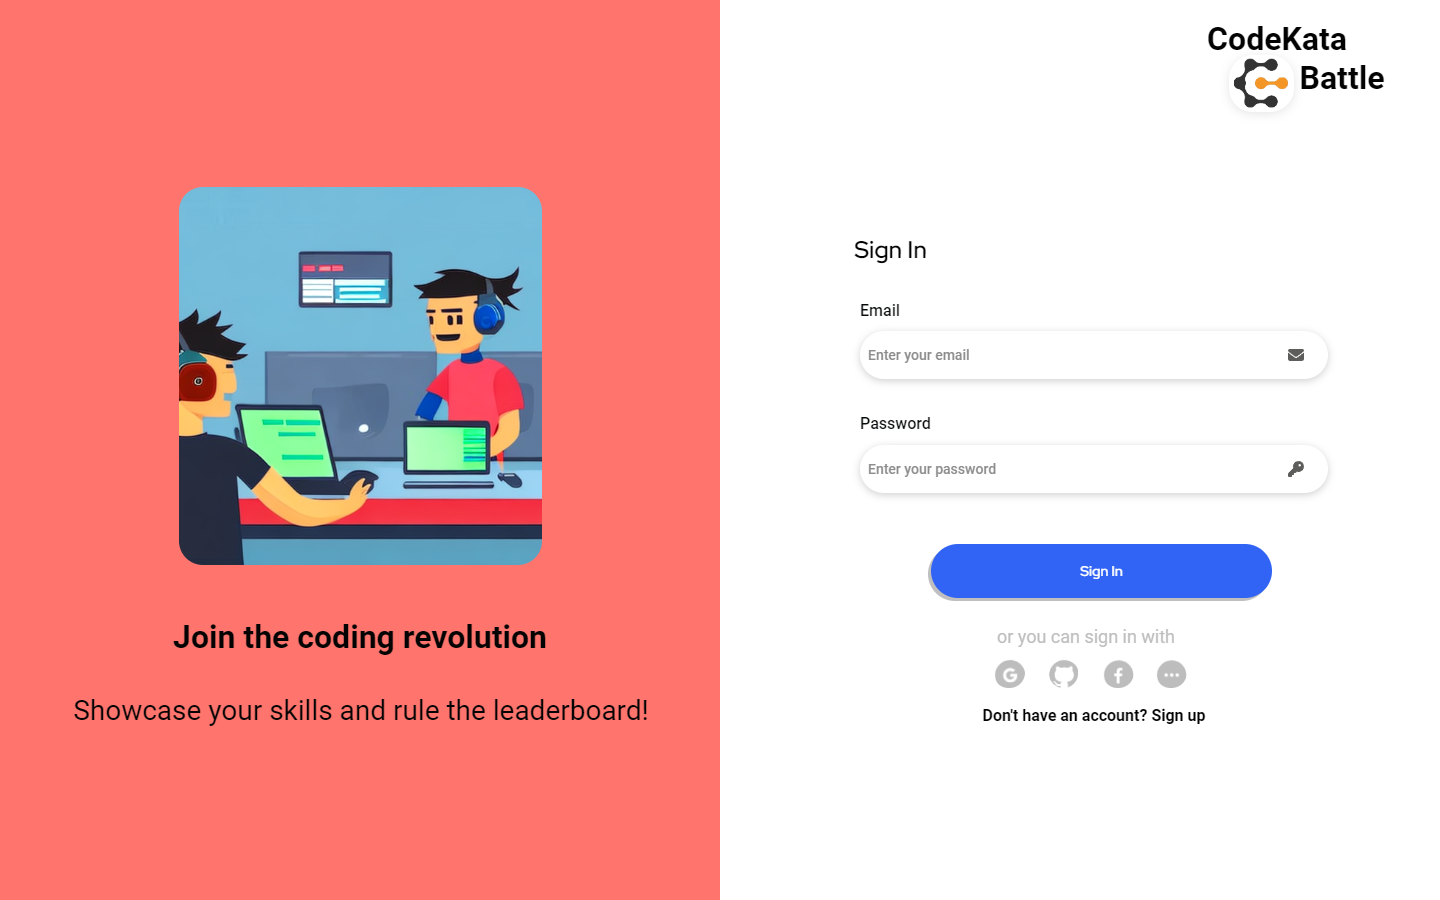
\includegraphics[width=0.8\textwidth]{Mockups/2_login.png}
        \caption{Login page}
    \end{figure}

    \item \textbf{Home page}\\
    The home page is the first page that the user sees after logging in. If the logged user is a student, the homepage contains a brief overview of platform's ongoing tournaments, battles the user is participating in, a calendar with upcoming deadlines and some statistics of past battles. Educator's homepage is similar, but will include some information about tournaments and battles he is responsible of. \\
    \begin{figure}[H]
        \centering
        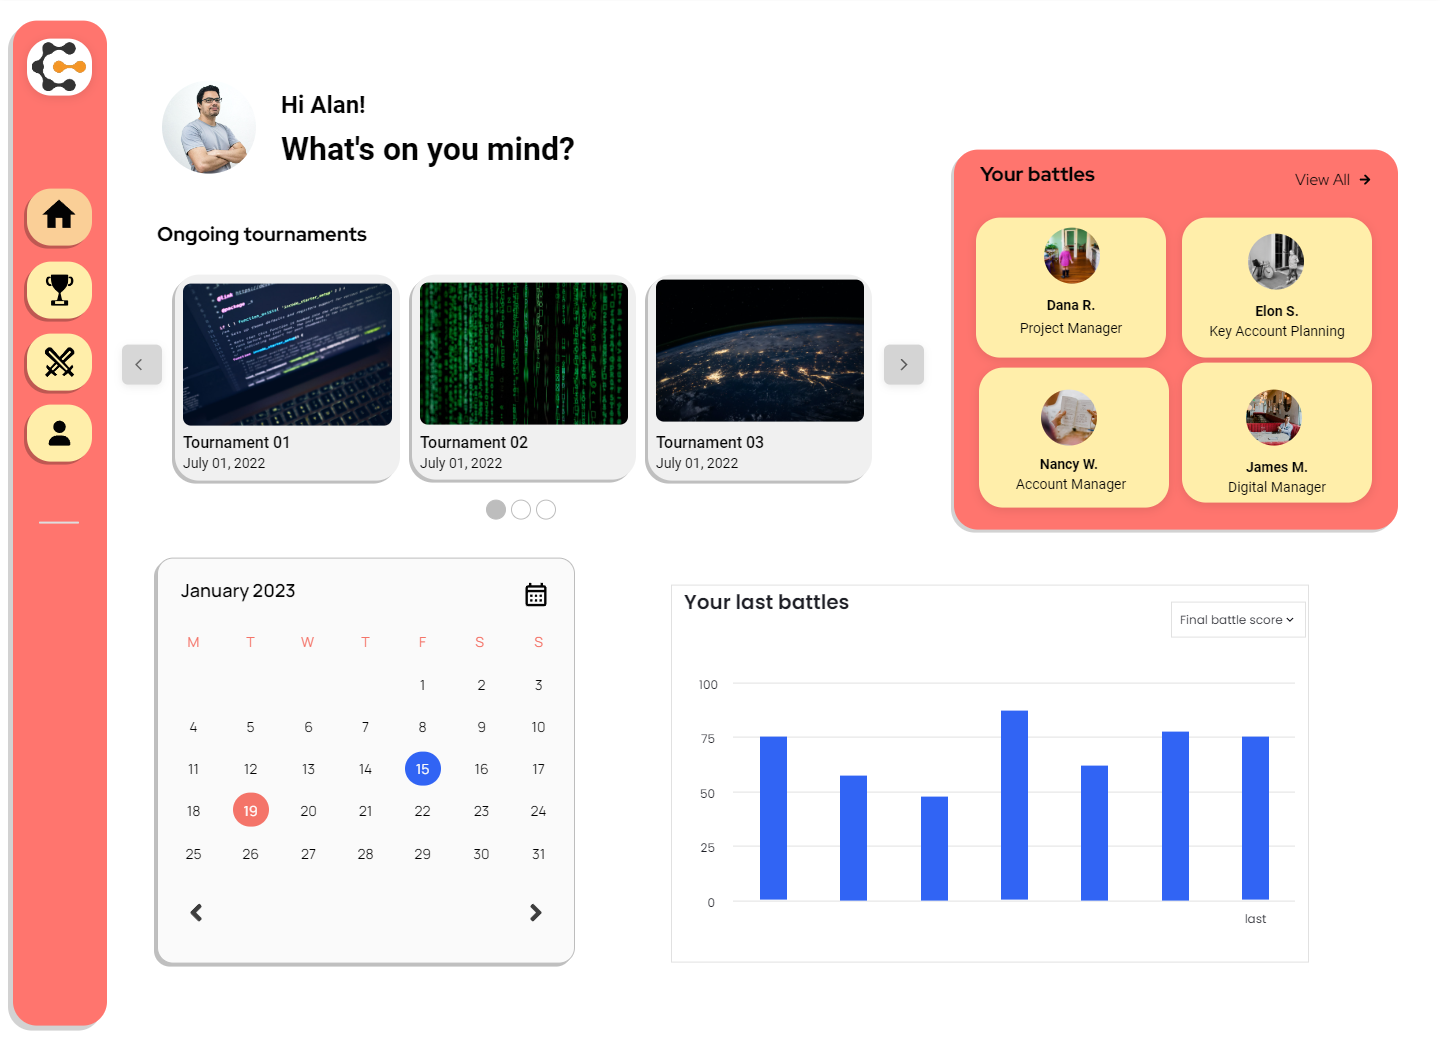
\includegraphics[width=0.8\textwidth]{Mockups/3_student_homepage.png}
        \caption{Home page from the perspective of an user logged as student}
    \end{figure}

    \item \textbf{Tournaments}\\
    The tournaments section will provide to the student a list of all ongoing tournaments in the platform and a list with all tournaments the student is enrolled in. The page will contain also some collections, to access for example popular tournaments or all past tournaments. By clicking on a tournament, the user will be redirected to the tournament page.\\ 
    \begin{figure}[H]
        \centering
        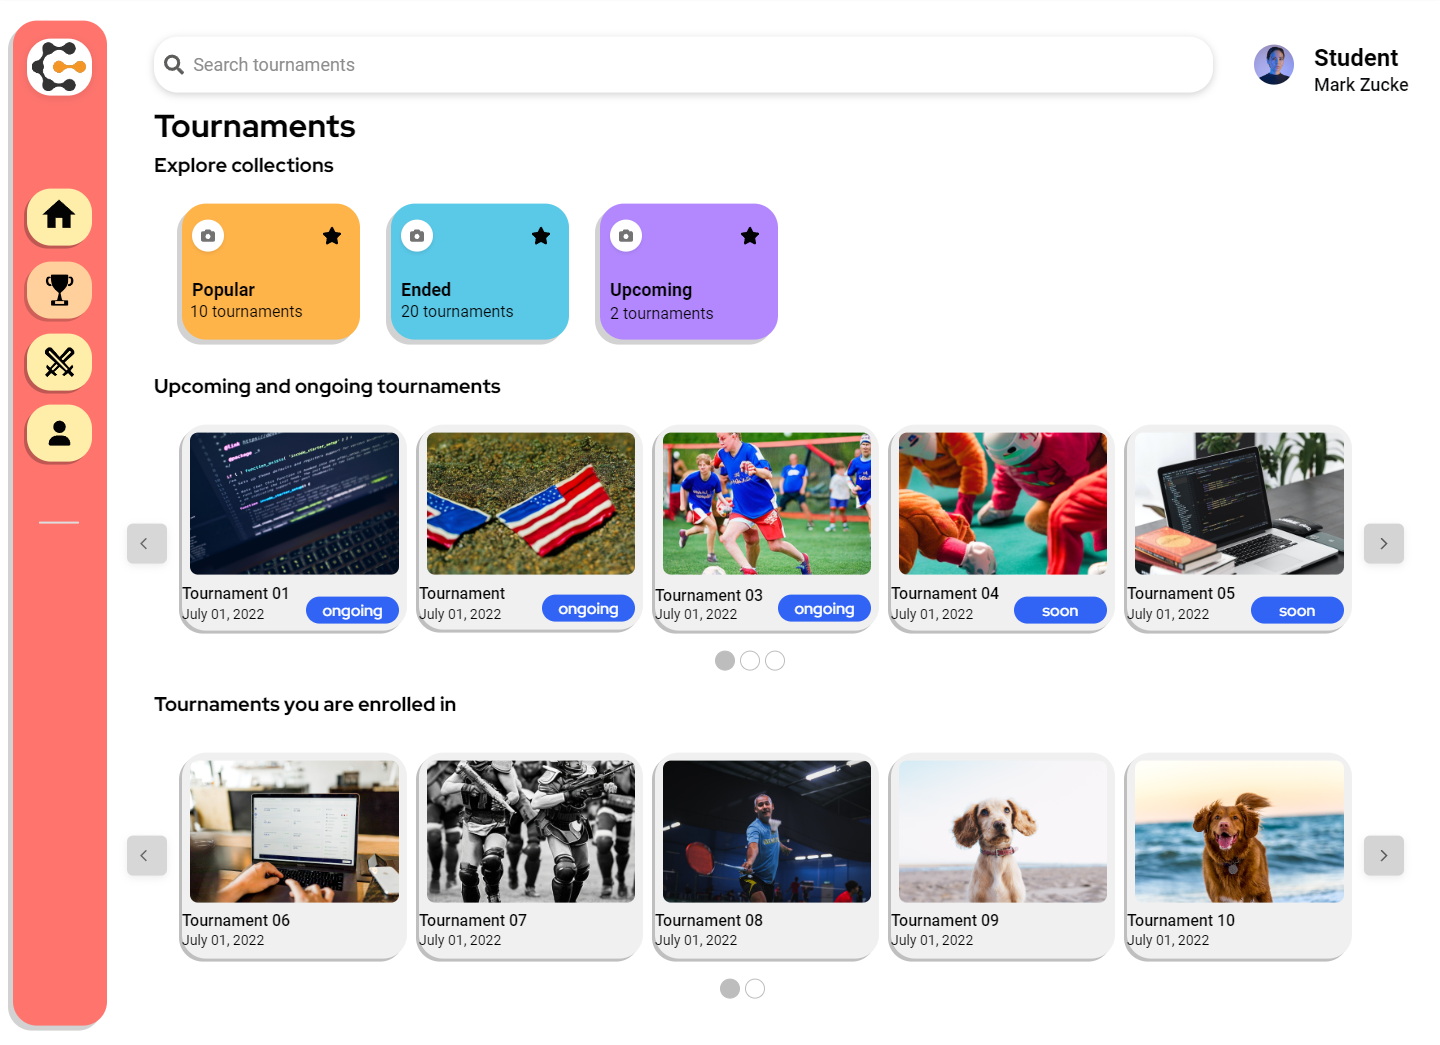
\includegraphics[width=0.8\textwidth]{Mockups/4_student_tournaments.png}
        \caption{Tournaments page from the perspective of an user logged as student}
    \end{figure}
    The corresponding page for educators will show basic similar information about tournaments, but will also provide a button to create a new tournament.\\
    \begin{figure}[H]
        \centering
        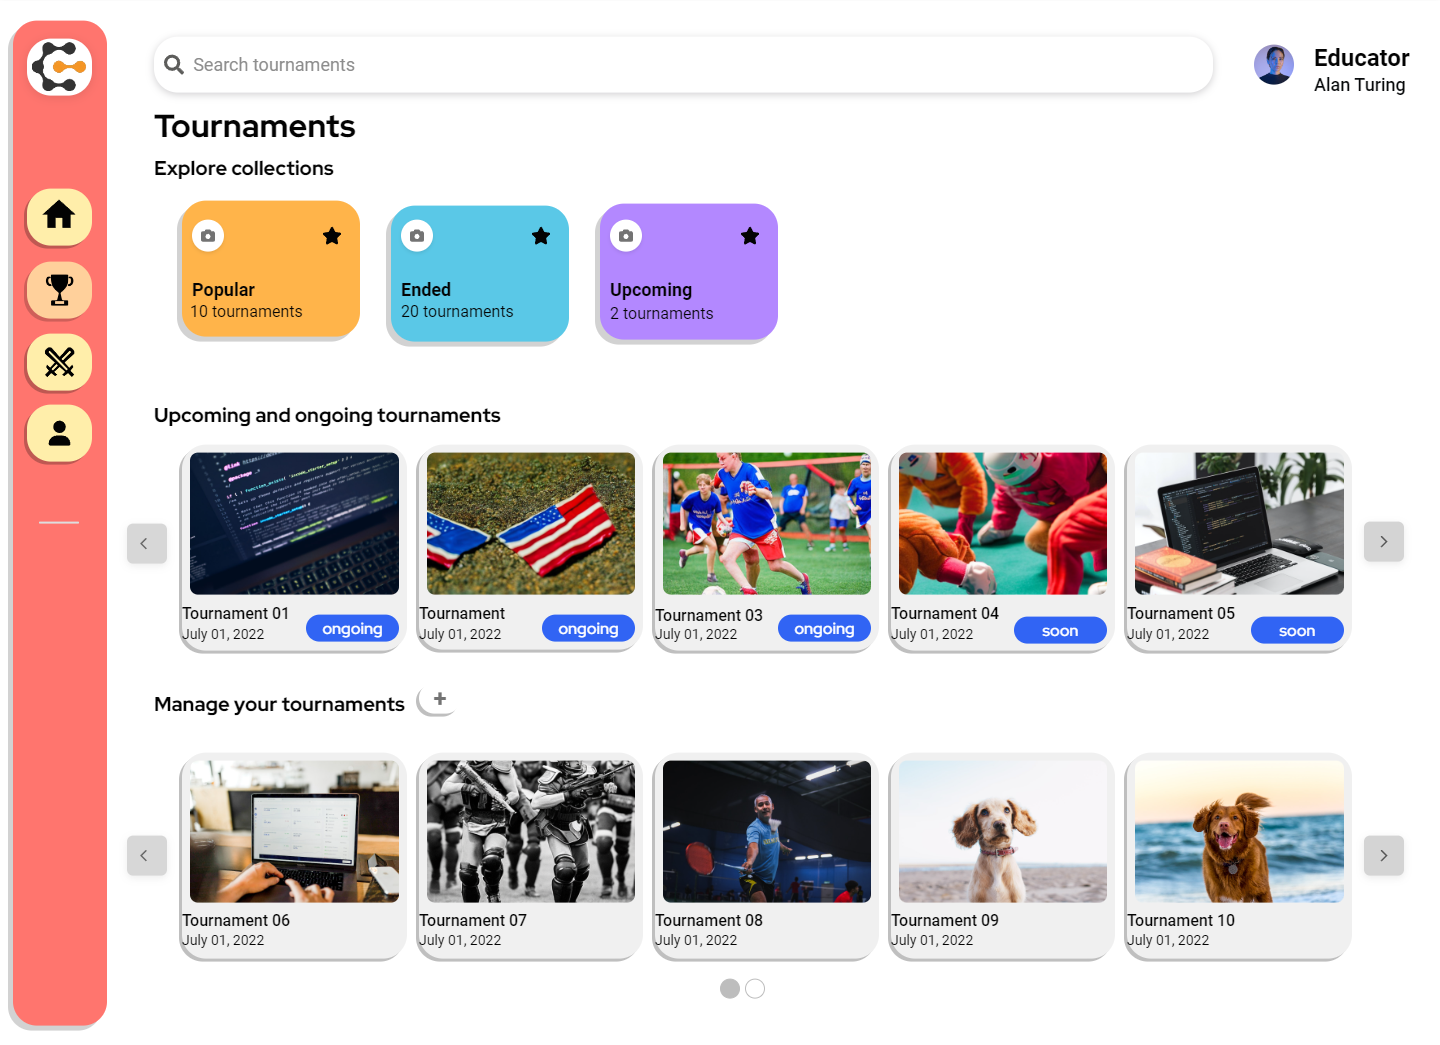
\includegraphics[width=0.8\textwidth]{Mockups/5_educator_tournaments.png}
        \caption{Tournaments page from the perspective of an user logged as educator}
    \end{figure}
    \begin{figure}[H]
        \centering
        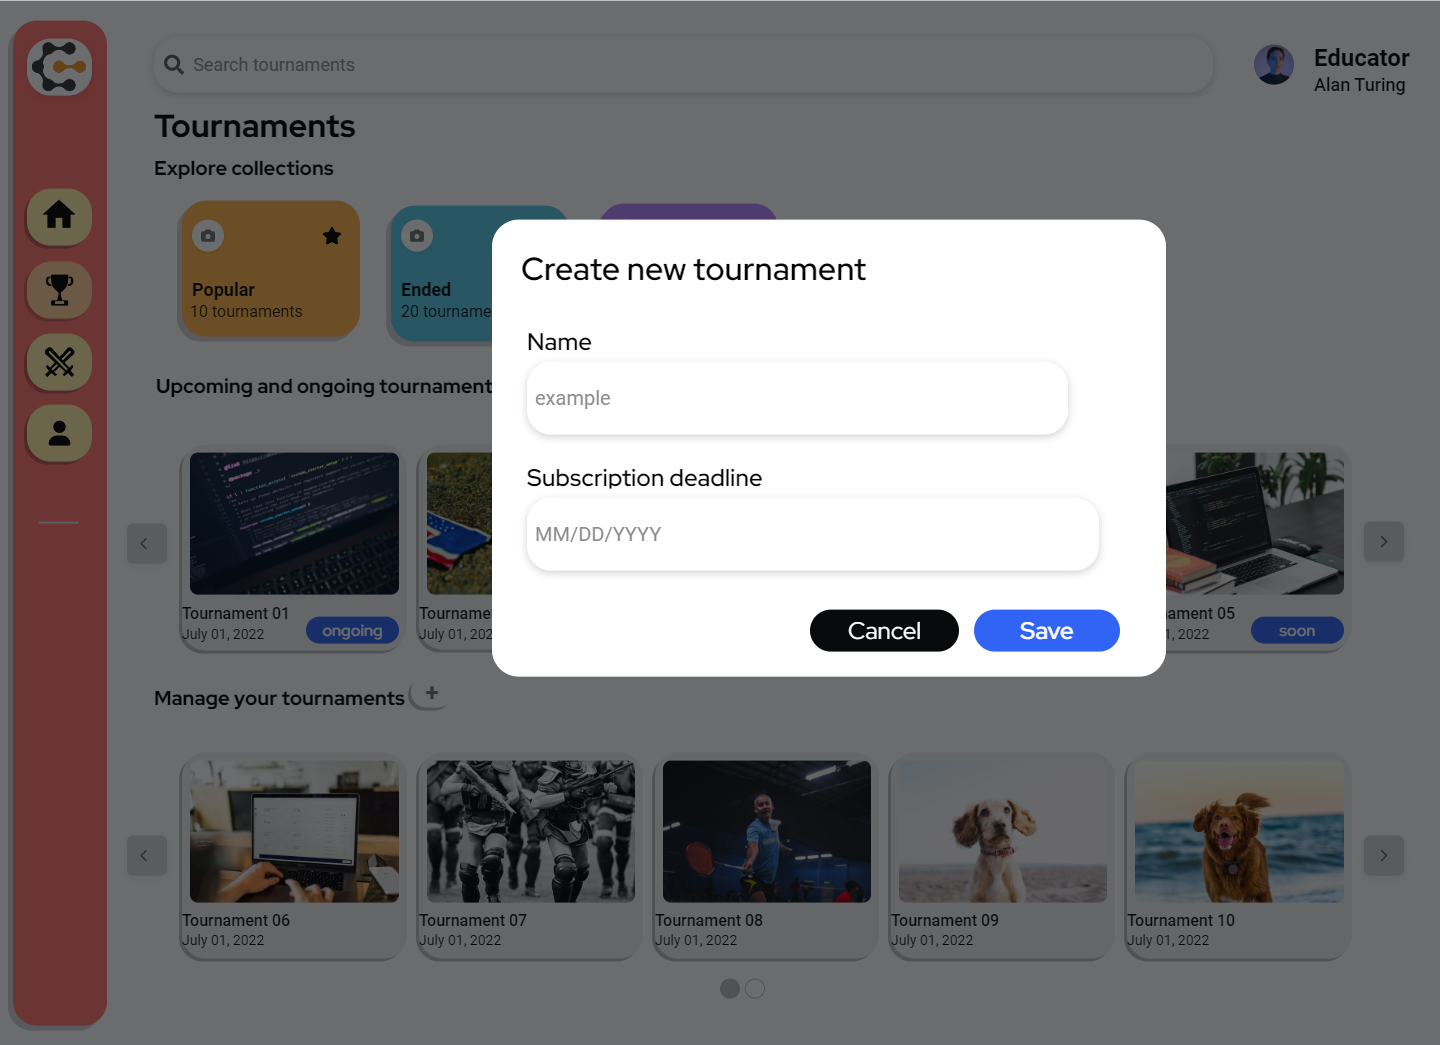
\includegraphics[width=0.8\textwidth]{Mockups/6_educator_create_tournament.png}
        \caption{Page used from educators to create a new tournament}
    \end{figure}
    The tournament page offers to the educator owning the tournament the possibility to manage it. He will be able to click the "Add collaborator" button to add another educator to the tournament by email address. Moreover, the page offers the "collaborators" tab that can be used to check and manage the list of collaborators. The last tab called "leaderboard" allows the educator to check the ranking of the students enrolled in the tournament. However, the main tournament page contains the list of all the battles created within the tournament.  By clicking on a specific battle, the educator will be redirected to the battle's page. Most importantly, the educator can create a battle by clicking on "Create battle" button.\\
    The student's tournament page will share most of the content, but the options to manage the tournament. The same page, if the tournament is not started yet, offers the possibility to the student to subscribe to the tournament and by default shows a list of partipants. \\
    \begin{figure}[H]
        \centering
        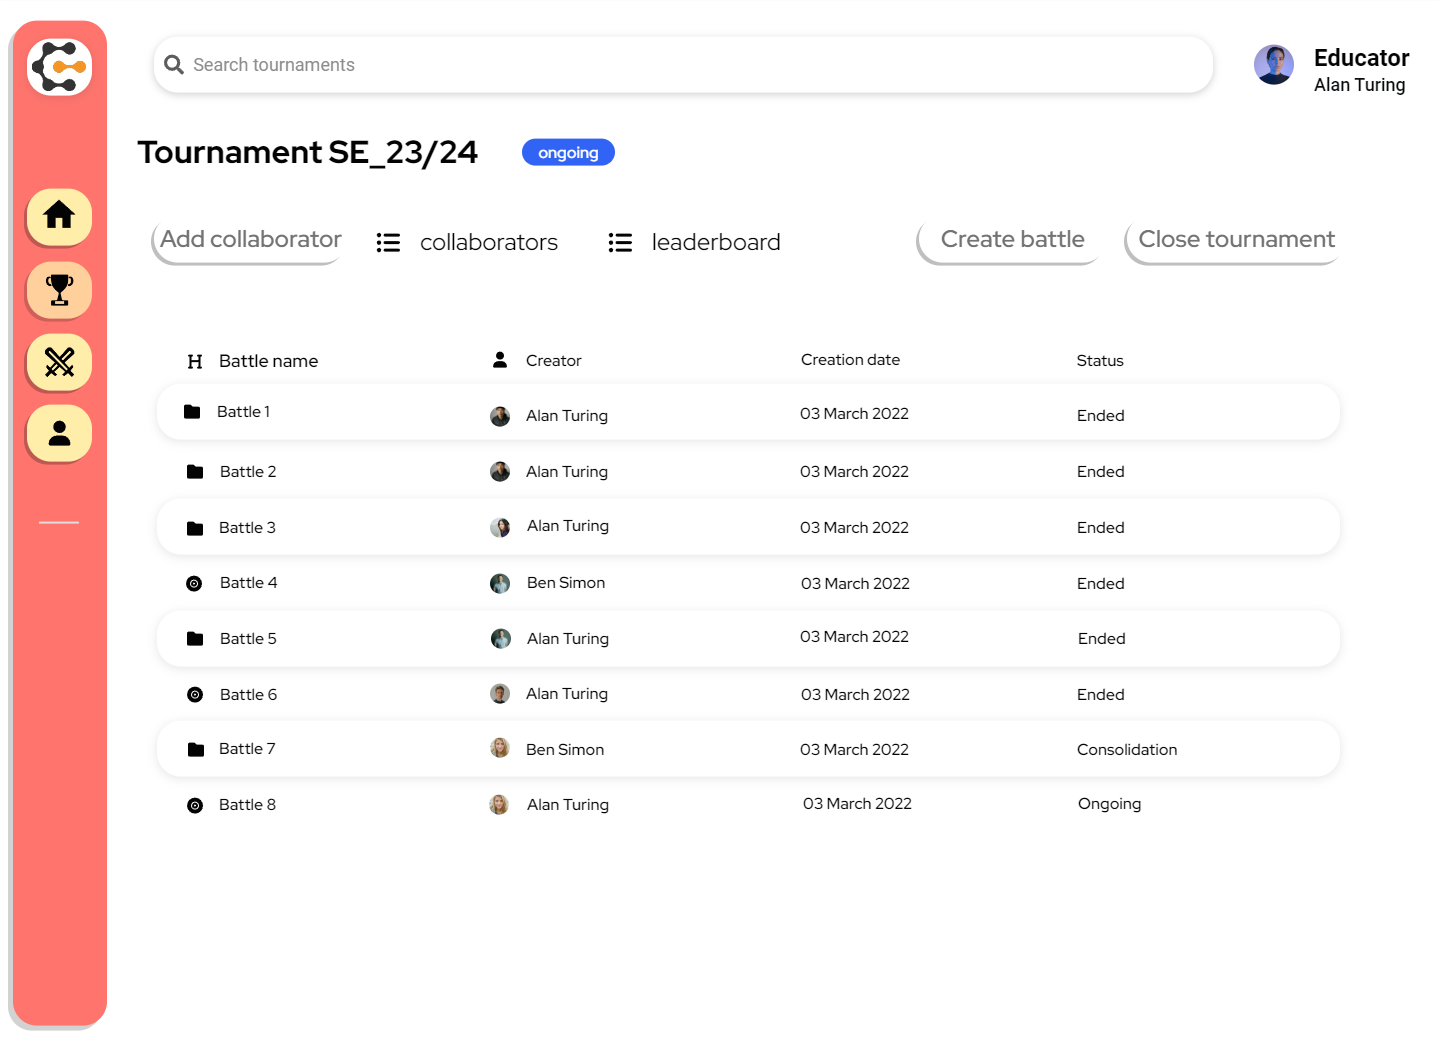
\includegraphics[width=0.8\textwidth]{Mockups/7_educator_manages_tournament.png}
        \caption{Page used from educators to manage the main settings of an ongoing tournament}
    \end{figure}
    \begin{figure}[H]
        \centering
        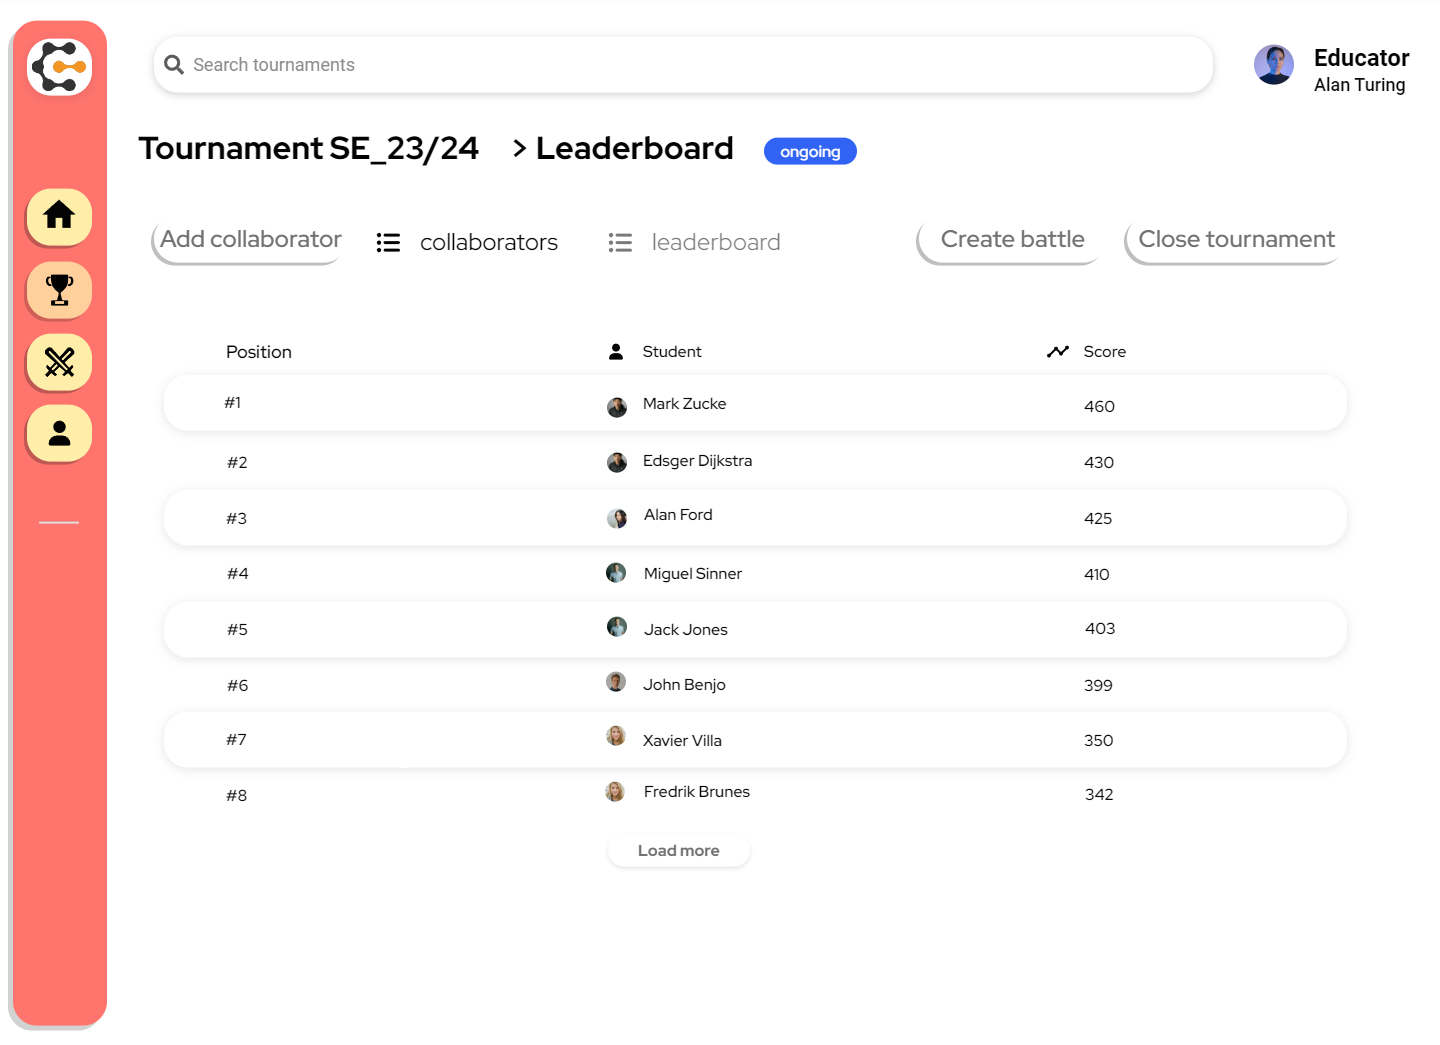
\includegraphics[width=0.8\textwidth]{Mockups/8_educator_tournament_leaderboard.png}
        \caption{"leaderboard" tab available to both educators and students to check the ranking in tournament}
    \end{figure}

    \begin{figure}[H]
        \centering
        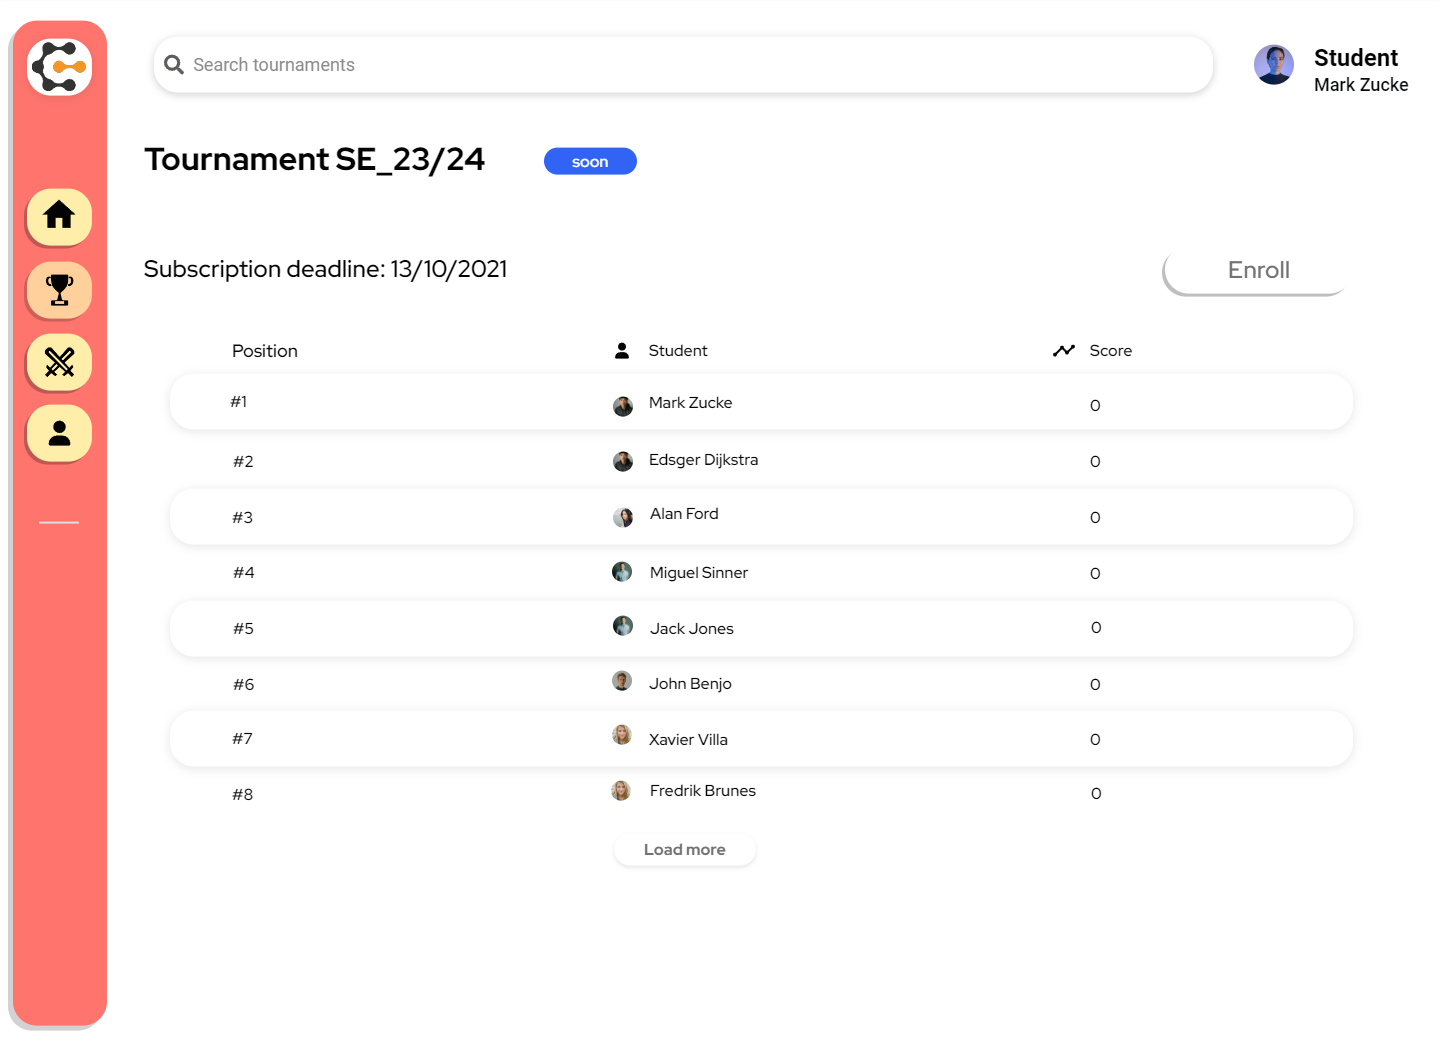
\includegraphics[width=0.8\textwidth]{Mockups/9_student_tournament_subscription.png}
        \caption{Page used from students to subscribe to a tournament}
    \end{figure}

    \item \textbf{Battles}\\
    After selecting the option to create a battle, the educator will be redirected to the page used to create a new battle. The page will ask the educator to provide the name of the battle, the description, the deadline for the registration and the deadline for the submission. Moreover, the educator will be able to select the minimum and maximum number of students per group allowed for the battle. The educator will be able to set some information about the battle and to configure the battle settings for the evaluation. He will be required to upload the Code Kata files of the battle, which contain the test cases and the basic template of the project that students will have to complete with their solutions.
    \begin{figure}[H]
        \centering
        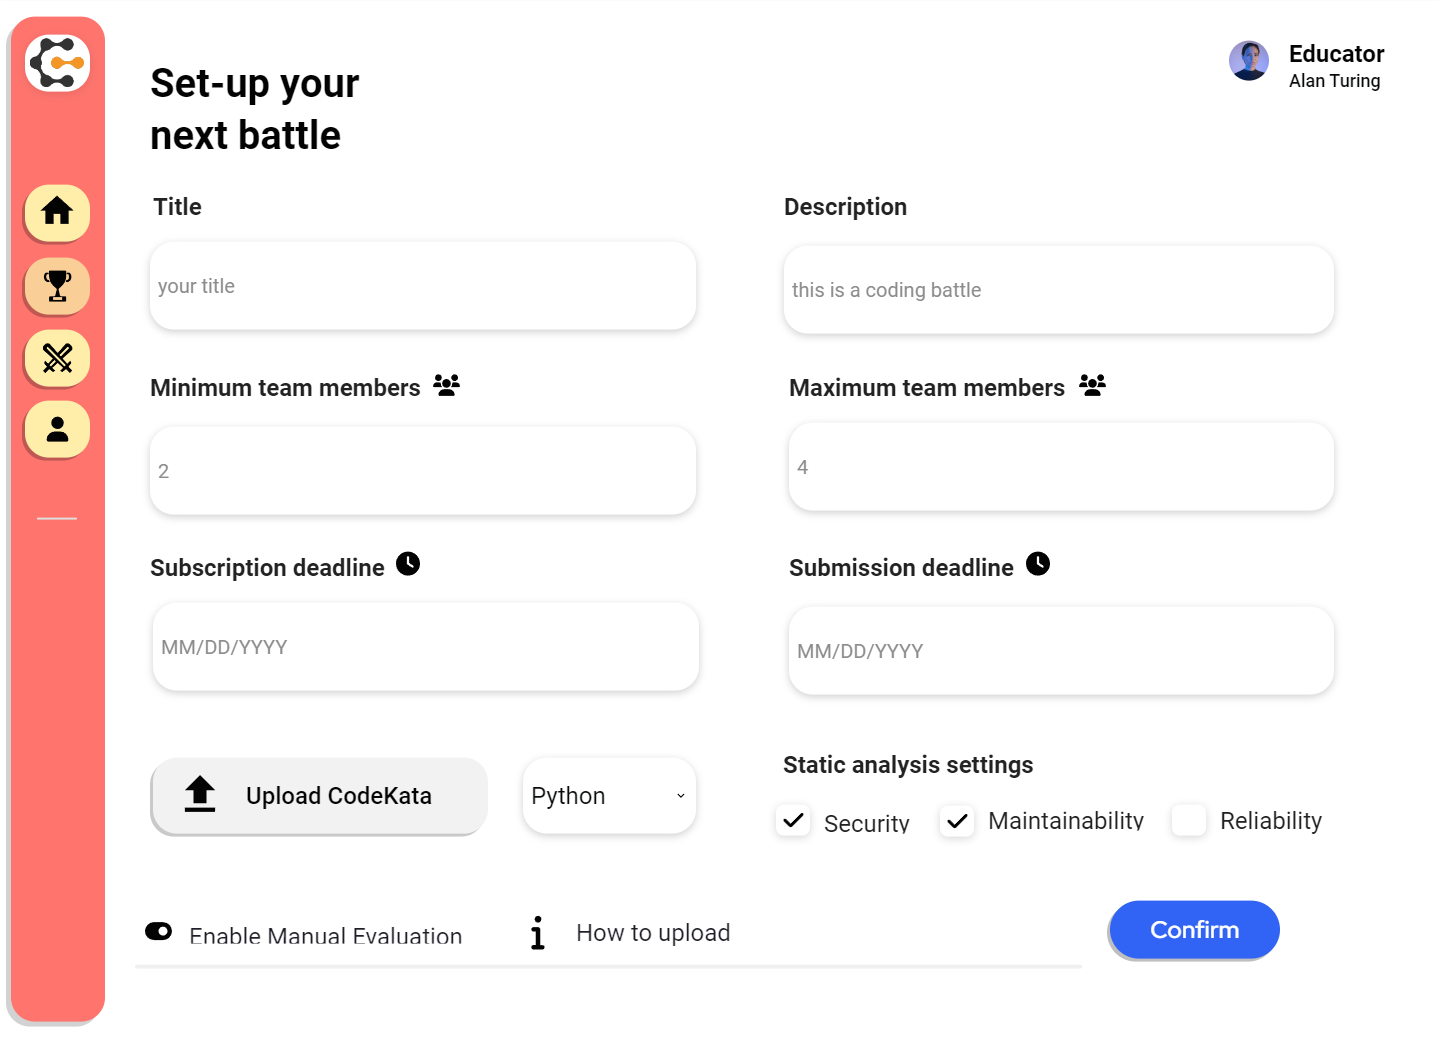
\includegraphics[width=0.8\textwidth]{Mockups/10_educator_create_battle.png}
        \caption{Page used from educators to create a new battle}
    \end{figure}
    When a battle is in subscription phase, the battle's page will offer to the student the options to subscribe to it by creating a new team or joining an already existing one. If the student decides to create the team, he will be asked to input the name of the team and its privacy setting. Instead, if the student want to join a team, the system will ask him to insert the name of the team (if public) or the invite code (if private). The page will also show the list of all the teams enrolled in the battle, to facilitate the team formation. Teams can be clicked in the leaderboard and a small pop-up with the list of members will be shown.\\
    \begin{figure}[H]
        \centering
        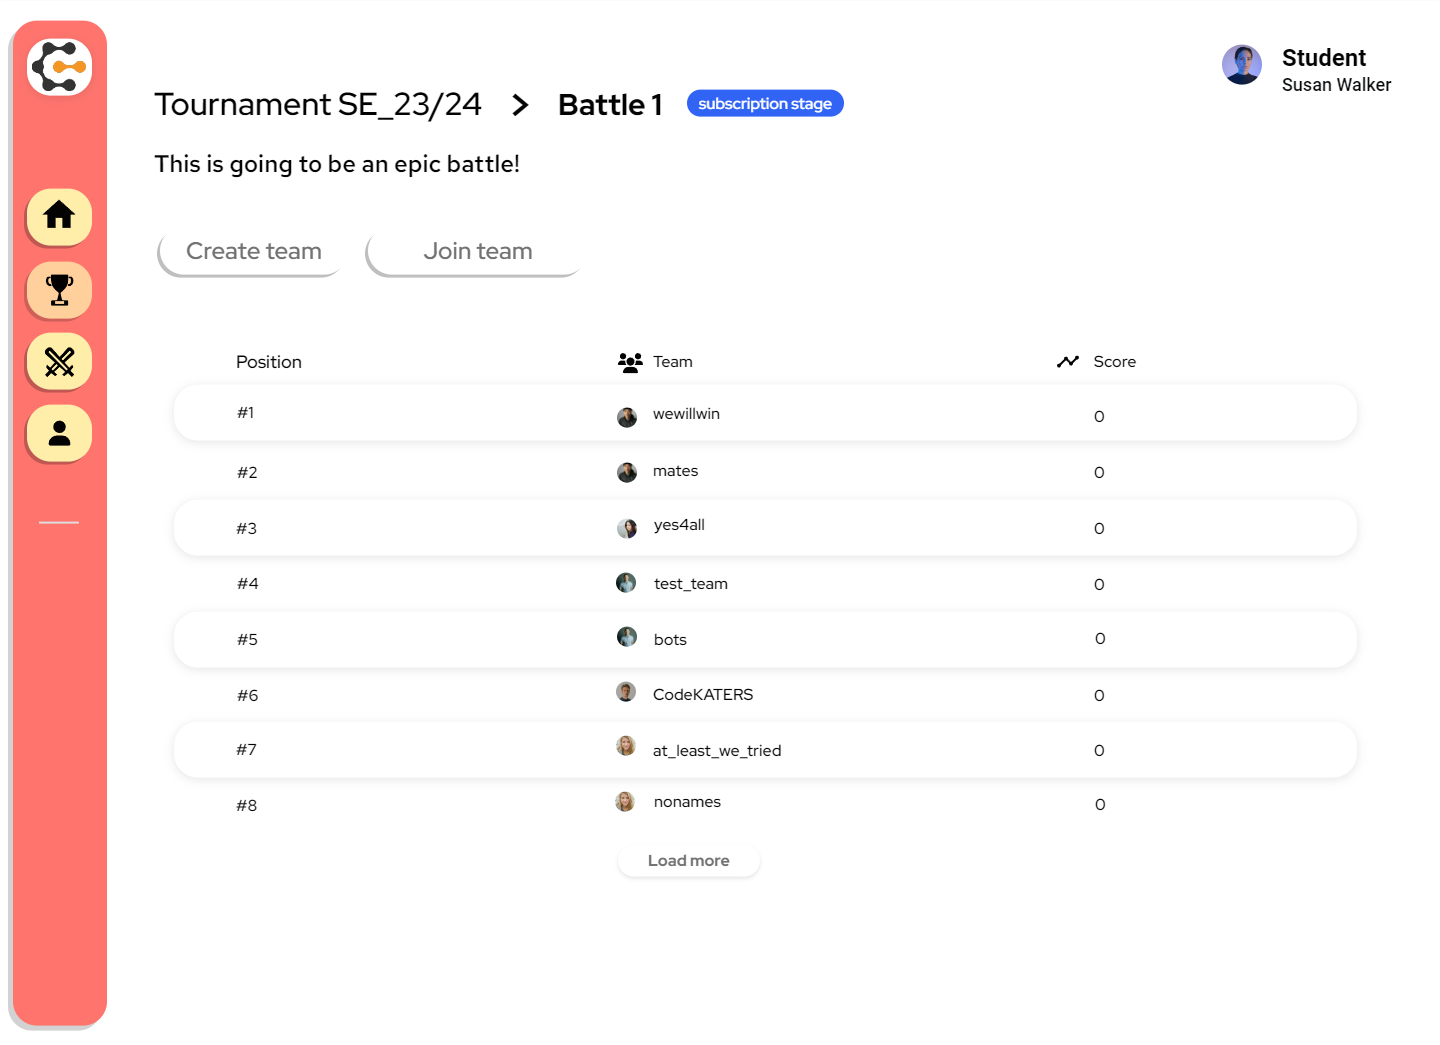
\includegraphics[width=0.8\textwidth]{Mockups/11_student_battle_subscription.png}
        \caption{Page used from students to subscribe to a battle}
    \end{figure}
    \begin{figure}[H]
        \centering
        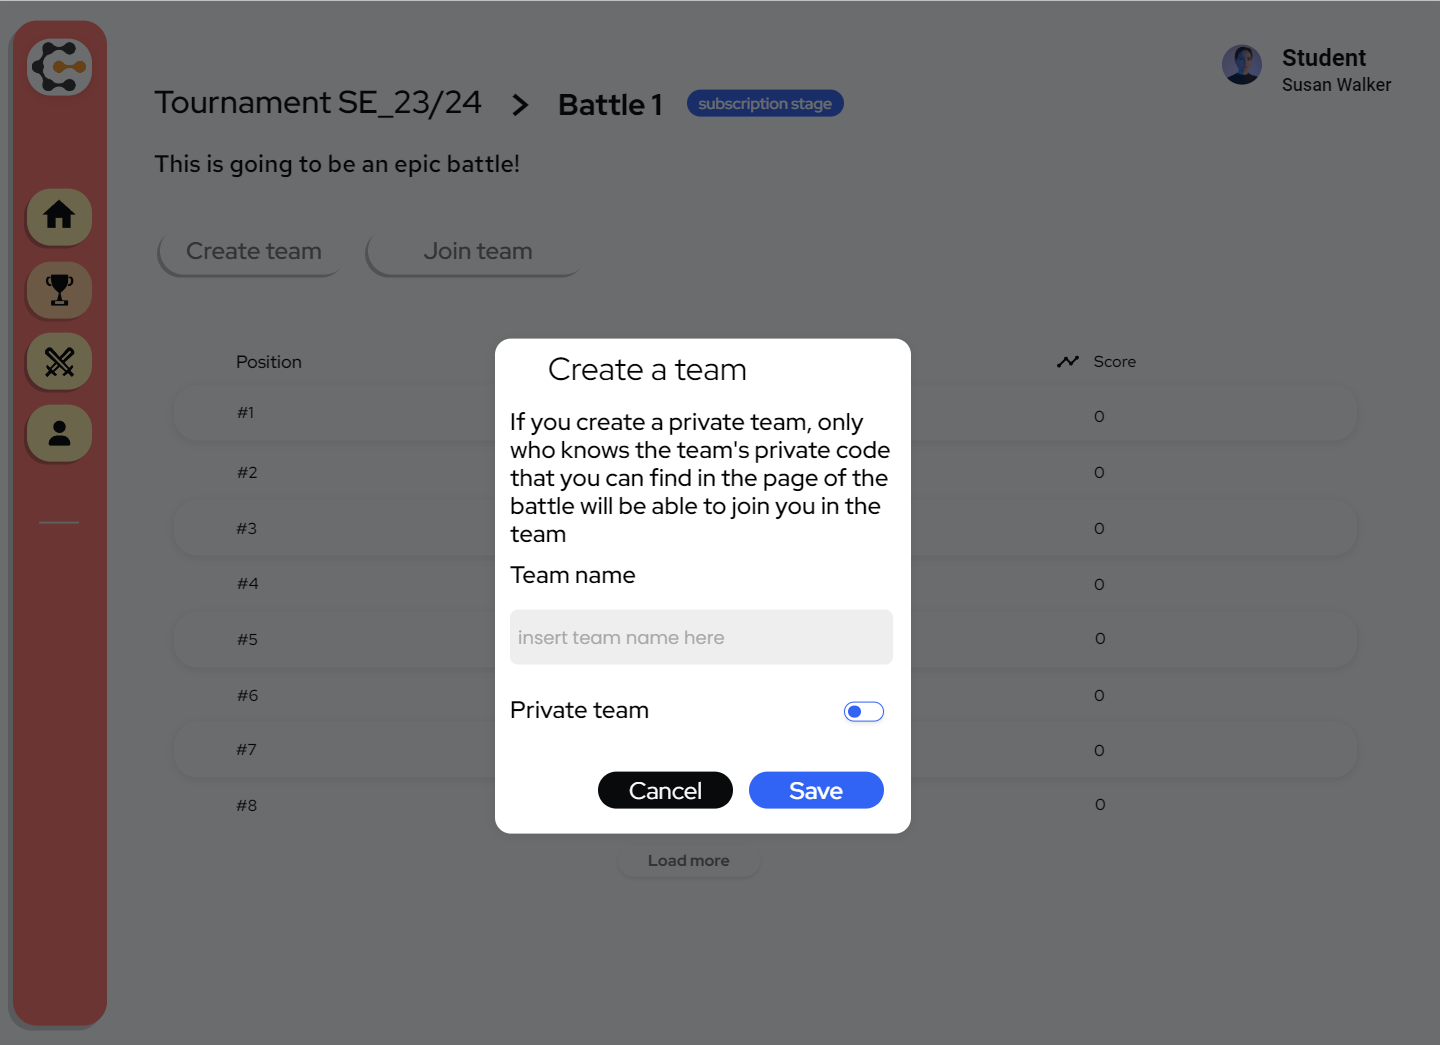
\includegraphics[width=0.8\textwidth]{Mockups/12_student_create_team.png}
        \caption{Page used from students to create a new team}
    \end{figure}
    \begin{figure}[H]
        \centering
        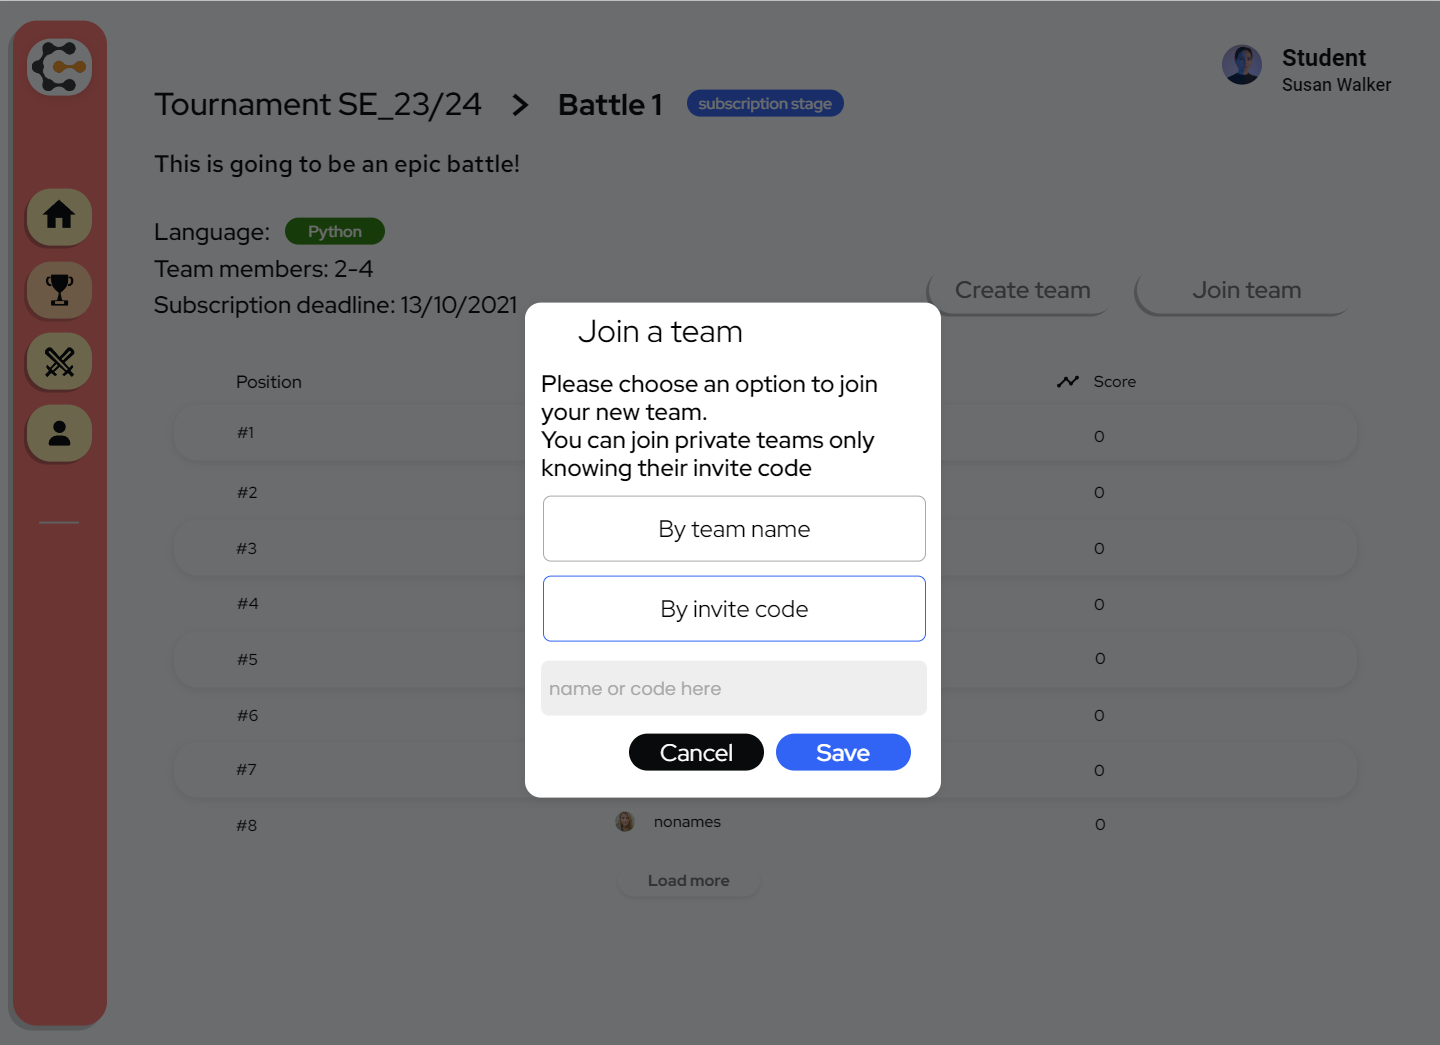
\includegraphics[width=0.8\textwidth]{Mockups/13_student_join_team.png}
        \caption{Page used from students to join a team}
    \end{figure}
    The page of a battle which is in the submission phase, will show by default the leadeboard of the teams. By clicking on "Your team" button, the student will be able access a section that contains important team settings and the information related to the submissions.\\
    In case the manual evaluation is not enabled, this page will have similar content for both educators and students, but the team settings button.\\

    \begin{figure}[H]
        \centering
        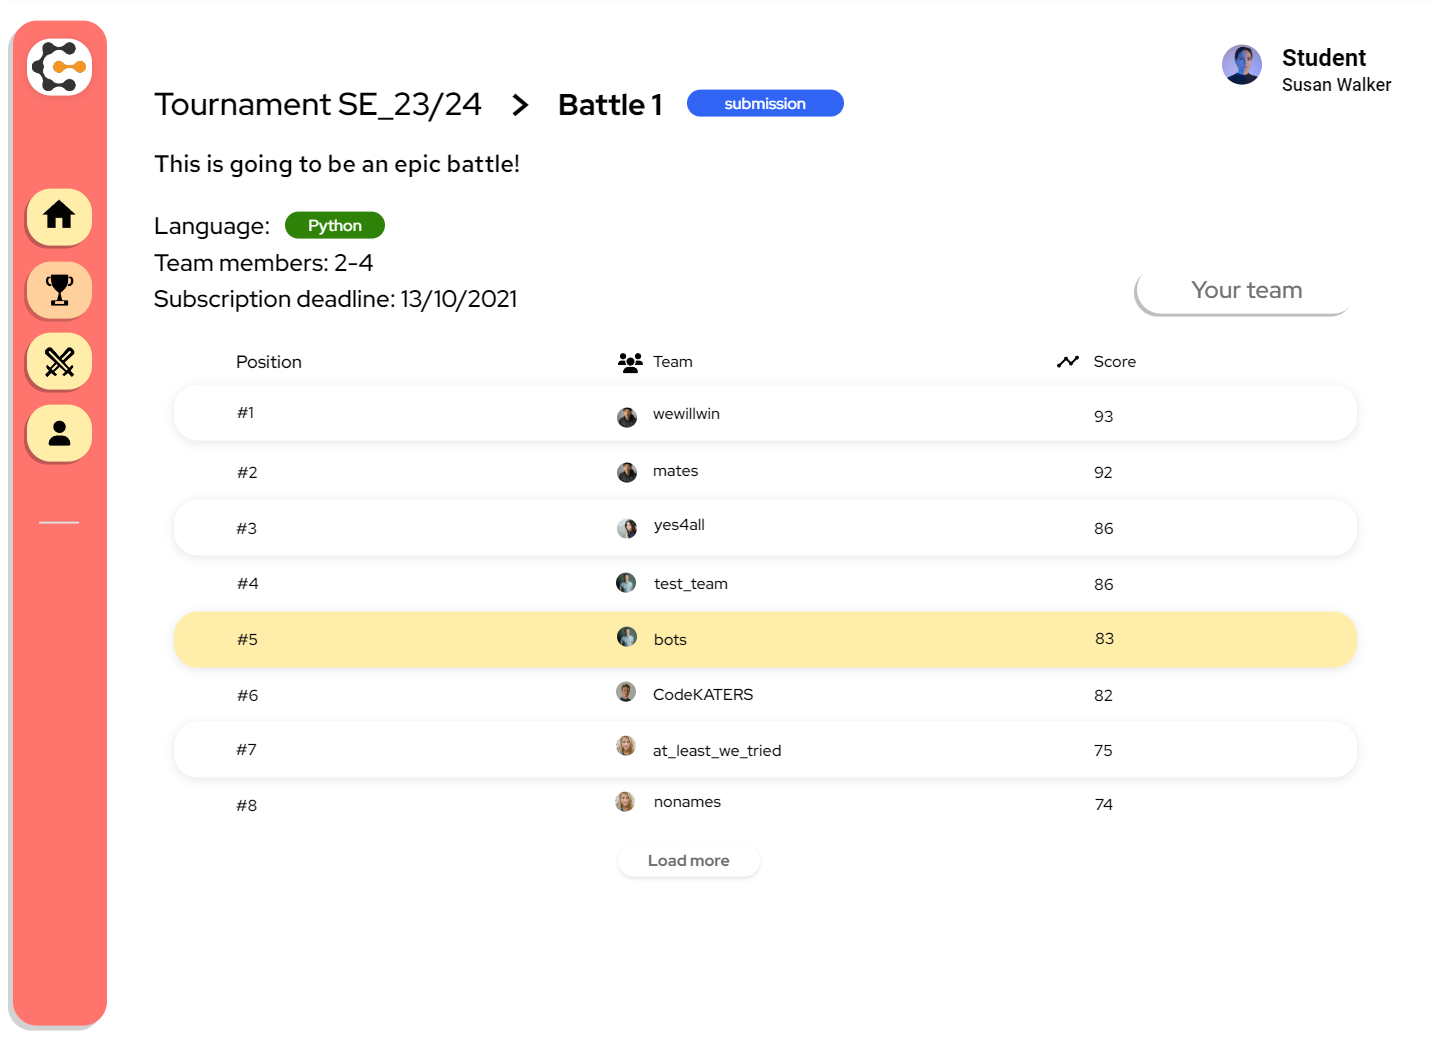
\includegraphics[width=0.8\textwidth]{Mockups/14_student_battle_submission.png}
        \caption{Page used from students when a battle is in submission phase}
    \end{figure}
    The team page, accessible only to students of team, will contain all important settings needed to properly setup the GitHub repository and evaluation information about the team's last submission. It will show also some statistics about past submissions to facilitate the tracking of the team's performances.
    By clicking on "Team members" box, the list of teammates will show up, with related commits count.\\
    \begin{figure}[H]
        \centering
        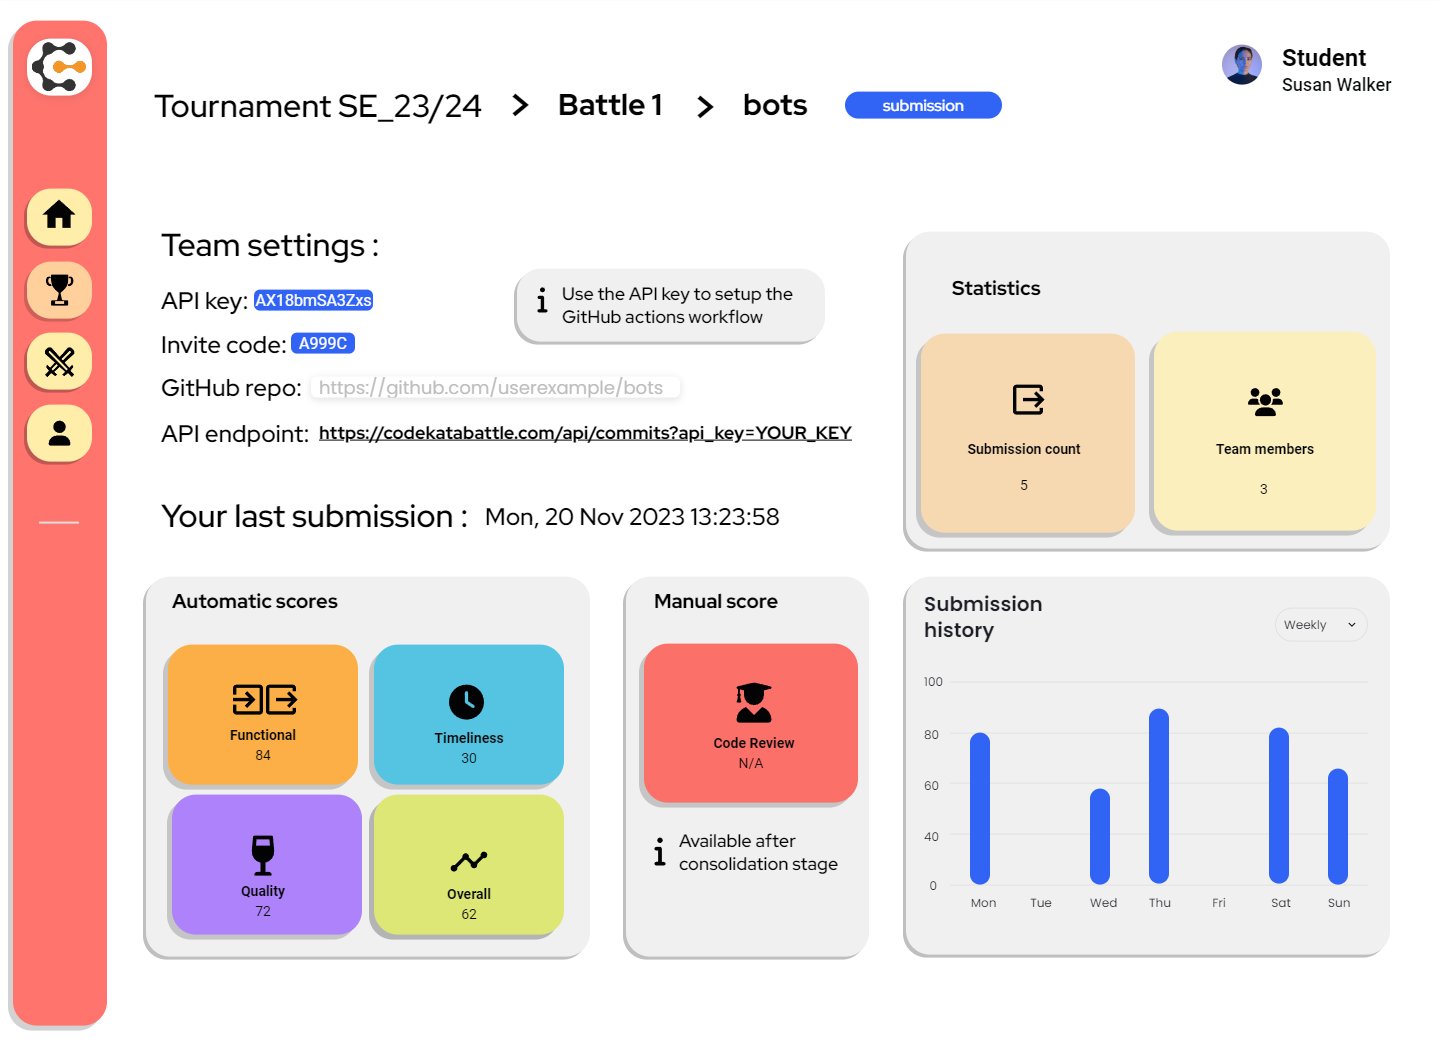
\includegraphics[width=0.8\textwidth]{Mockups/15_student_team.png}
        \caption{Page used from students to manage the settings of their team and to check submissions information}
    \end{figure}
    
    \item \textbf{Evaluation}\\
    The battle page, during the optional consolidation stage, will offer a special team leaderboard, with an overview of both manual and automatic scores. By clicking on a specific team, the educator has access to the evaluation page of the team. The page also contains a button to close the consolidation phase once the educator has evaluated all the teams.\\
    In the evaluation section, the educator is able to access the GitHub repository of the team to check the code of the last submission. Finally, he is provided with a field to input the manual score.
    \begin{figure}[H]
        \centering
        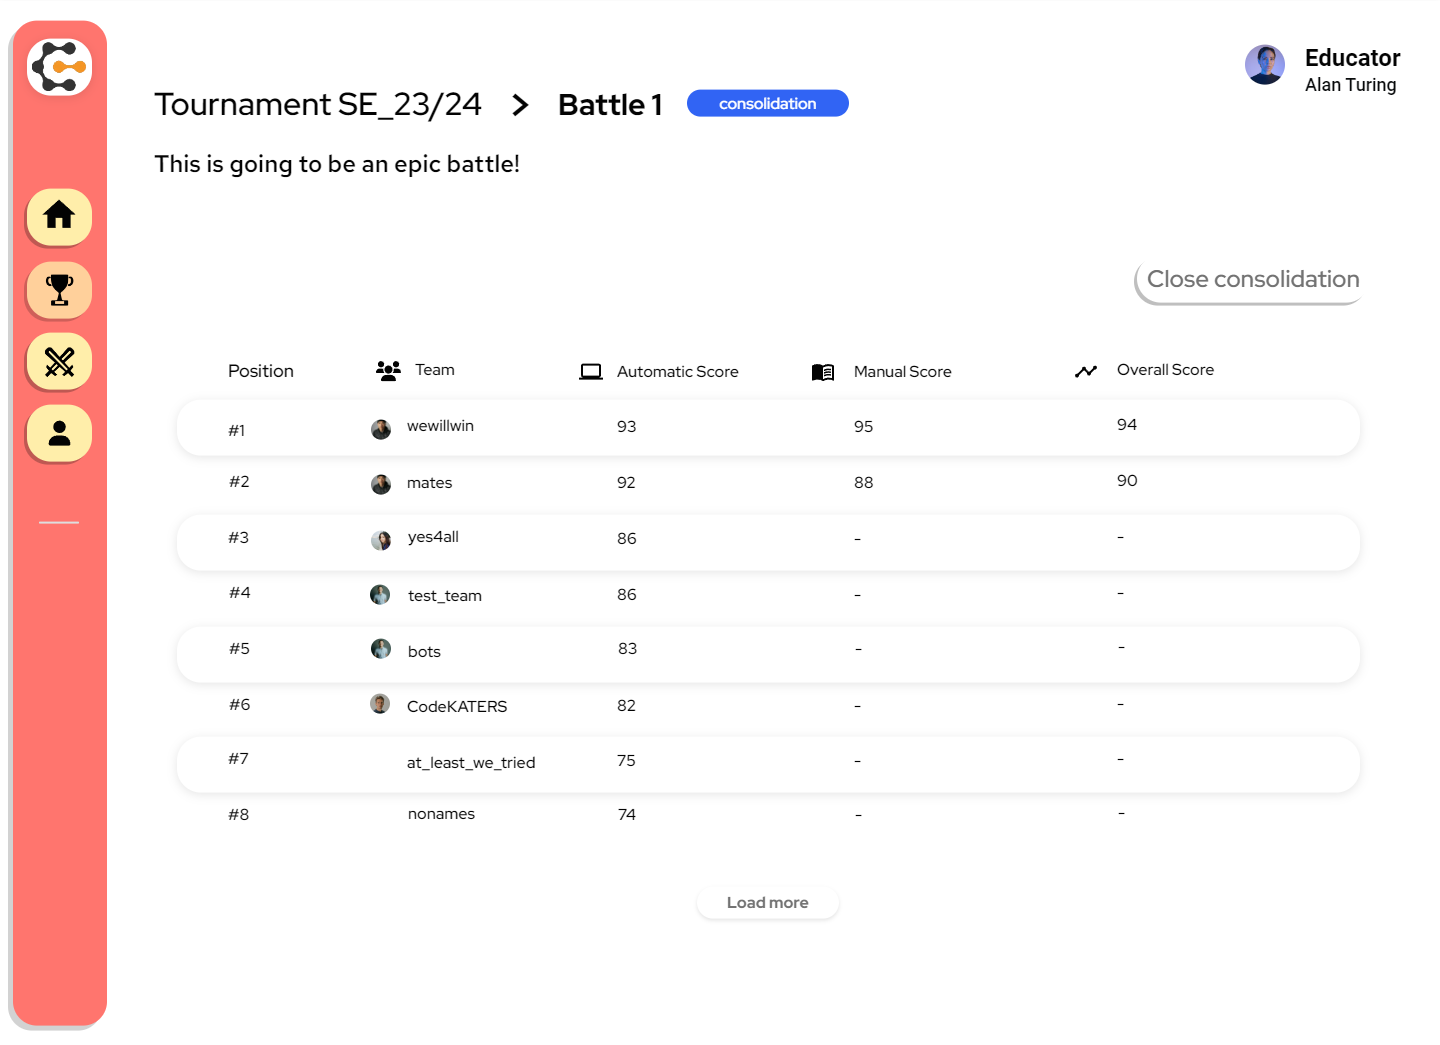
\includegraphics[width=0.8\textwidth]{Mockups/16_educator_battle_consolidation.png}
        \caption{Page used from educators to manage the consolidation stage of a battle}
    \end{figure}
    \begin{figure}[H]
        \centering
        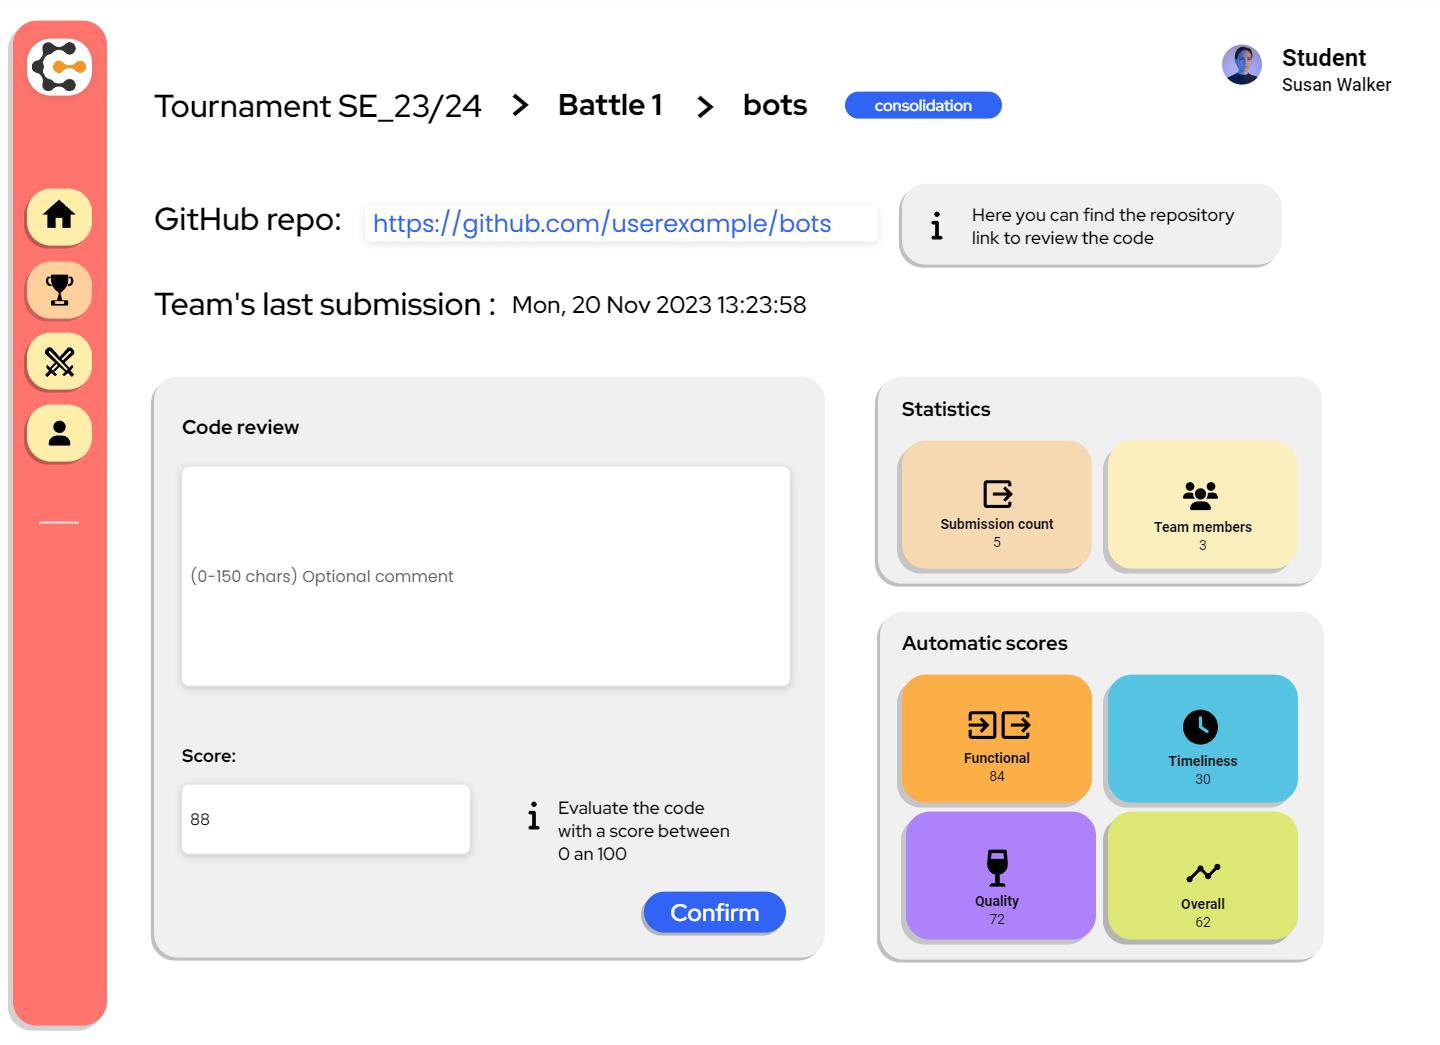
\includegraphics[width=0.8\textwidth]{Mockups/17_educator_manual.png}
        \caption{Page used from educators to manually evaluate a submission}
    \end{figure}
\end{enumerate}

\subsubsection{Hardware Interfaces}
The software does not require any other hardware interface different than personal computers or smartphones equipped with modern browser from which users can access the platform.
\subsubsection{Software Interfaces}
Some of the functionalities provided by the system exploit specific interfaces to work. These are:
\begin{itemize}
    \item \textbf{GitHub interface}: the system must be able to interface with GitHub API to create the original repository for each battle and to pull code submissions.
    \item \textbf{Static analysis tools}: some of the aspects that have to be evaluated require the execution of some static analysis method over the provided code. In this case, the platform utilizes external services directly provided by third-party organizations. The external services must support the set of languages supported by CKB the platform.
\end{itemize}
Each of these interfaces are implemented by correctly setting and utilizing specific API calls to the involved services that will be included inside the platform’s inner processes.

Moreover, in order to be notified about the submission of a new solution, the system itself must expose a REST endpoint that will be invoked by the automated GitHub Actions workflow set up by each team on their repository.
\subsubsection{Communication Interfaces}
Given that the majority of the system's services are provided through the platform's website and REST API calls, no other protocol than HTTP should be needed. Anyway, it is worth mentioning that part of the communication between the system and user is achieved through notifications sent via mail using an external mail service provider.

\subsection{Functional Requirements}
The main requirements the system has to fulfill are the following:
\begin{enumerate}[label=$\bullet$ \textbf{R\arabic*:}]
    \item System shall allow user to register as educator or student.
    \item System shall allow user to log in.
    \item System shall allow educator to create a tournament.
    \item System shall allow educator (tournament creator) to set the name of the tournament.
    \item System shall allow educator (tournament creator) to set the subscription deadline of the tournament.
    \item System shall notify all students enrolled to the platform about a newly created tournament.
    \item System shall allow educator (tournament creator) to end the tournament.
    \item System shall allow educator (tournament creator) to add another educator as collaborator to the tournament.
    \item System shall allow educator (tournament creator or collaborator) to create a battle for the tournament.
    \item System shall allow educator (battle creator) to upload the Code Kata of the battle.
    \item System shall allow educator (battle creator) to set minimum and maximum number of students per group allowed for the battle.
    \item System shall allow educator (battle creator) to set the registration deadline of the battle.
    \item System shall allow educator (battle creator) to set the submission deadline of the battle.
    \item System shall allow educator (battle creator) to enable/disable optional manual evaluation for the battle.
    \item System shall allow educator (battle creator) to select relevant aspects of code quality to be extracted through static analysis.
    \item System shall notify all users enrolled to a tournament about a newly created battle.
    \item The system shall be able to perform static analysis on submitted code utilizing third-party static code analysis tools and services.
    \item System shall create the GitHub repository of a battle as soon as the registration phase closes, sending its link to all involved students.
    \item System shall assign to each submission sent before the submission deadline a score (natural number between 0 and 100) combining correctness, timeliness and code quality \textit{as soon as possible}.
    \item System shall allow educator (battle creator) to set a manual score (natural number between 0 and 100) to the last valid team’s submission during the consolidation stage of the battle.
    \item System shall compute a final score combining automatic and manual score (if available) for each team if manual evaluation is enabled.
    \item System shall update the battle teams’ ranks right after a new score is available.
    \item System shall notify all students participating to the battle about the availability of the final battle rank.
    \item System shall update the tournament students’ scores as the sum of all the battle scores received during the tournament once the final battle rank becomes available.
    \item System shall notify all involved users about the availability of the tournament student’s final rank.
    \item System shall allow all users to see the list of ongoing tournaments.
    \item System shall allow all users to see all tournaments’ ranks.
    \item System shall allow all users to see all battles' ranks.
    \item System should manage every ranking (tournament or battle) in a way that it represents the correct order of students/teams within its context, from the ones with the highest score to the ones with the lowest.
    \item System shall allow student to enroll to a tournament within the subscription deadline.
    \item System shall allow student to create a team within the registration deadline.
    \item System shall allow student (team creator) to set the team name.
    \item System shall allow student (team creator) to set the privacy of the group.
    \item System shall allow student to join a team \textit{only} before the registration deadline.
    \item System shall allow \textit{only} students who know the correct invite code to join private groups.
    \item System shall allow team members to set their the repository URL.
    \item System shall generate a unique API token for each team.
    \item System should offer an external API which, when invoked, will notify the platform about a new commit on a team’s GitHub repository.
    \item System shall allow the educator to access the code of the submitted solutions.
    \item System shall generate a unique invite code for each team.
    \item System shall allow educator (battle creator) to close the consolidation stage of the battle if manual evaluation is enabled.
    \item System shall allow students to see the latest score of their team.
\end{enumerate}
\subsubsection{Use cases}
\begin{center}
    \begin{tabular}{ |c|m{10cm}| }
        \hline
        \textbf{ID} & 1 \\
        \hline
        \textbf{Name} & User registration \\
        \hline
        \textbf{Actors} & Unregistered user \\
        \hline
        \textbf{Entry conditions} & The user has opened the webapp. \\
        \hline
        \textbf{Event flow} &
        \begin{enumerate}
            \item The user opens the webapp.
            \item The user clicks on the "Sign up" button.
            \item The user fills the form with his personal information.
            \item The user clicks on the "Sign up" button.
            \item The system checks if the provided information is valid.
            \item The system creates a new user account.
            \item The system redirects the user to the home page.
        \end{enumerate} \\
        \hline
        \textbf{Exit conditions} & The user has successfully created a new account. \\
        \hline
        \textbf{Exceptions} & 
        \begin{itemize}
            \item The user has provided invalid information.
            \item The user has provided an email address already used by another account.
        \end{itemize} \\
        \hline
        \textbf{Alternative} &
        \begin{enumerate}
            \item The user opens the webapp.
            \item The user clicks on the "Sign up with Google" button.
            \item The user is redirected to the Google login page.
            \item The user logs in with his Google account.
            \item The system checks if the provided information is valid.
            \item The system creates a new user account.
            \item The system redirects the user to the home page.
        \end{enumerate} \\
        \hline
    \end{tabular}
\end{center}

\subsubsection{Goals mapping}
$\bullet$ \textbf{G1}: Allow students to participate to collaborative programming challenges
\begin{center}
    \begin{tabular}{ |m{3cm}|m{10cm}| }
        \hline
        \textbf{Requirements} 
        & \textbf{R1}: System shall allow user to register as educator or student \\
        & \textbf{R2}: System shall allow user to log in \\
        & \textbf{R6}: System shall notify all students enrolled to the platform about a newly created tournament \\
        & \textbf{R16}: System shall notify all users enrolled to a tournament about a newly created battle \\
        & \textbf{R18}: System shall create the GitHub repository of a battle as soon as the registration phase closes, sending its link to all involved students \\
        & \textbf{R26}: System shall allow all users to see the list of ongoing tournaments \\
        & \textbf{R30}: System shall allow student to enroll to a tournament within the subscription deadline \\
        & \textbf{R31}: System shall allow student to create a team within the registration deadline \\
        & \textbf{R32}: System shall allow student (team creator) to set the team name \\
        & \textbf{R33}: System shall allow student (team creator) to set the privacy of the group \\
        & \textbf{R34}: System shall allow student to join a team \textit{only} before the registration deadline \\
        & \textbf{R35}: System shall allow \textit{only} students who know the correct invite code to join private groups \\
        & \textbf{R36}: System shall allow team members to set their the repository URL \\
        & \textbf{R37}: System shall generate a unique API token for each team \\
        & \textbf{R38}: System should offer an external API which, when invoked, will notify the platform about a new commit on a team’s GitHub repository \\
        & \textbf{R40}: System shall generate a unique invite code for each team \\
        \hline
    \end{tabular}
    \begin{tabular}{ |m{3cm}|m{10cm}| }
        \hline
        \textbf{Domain \newline Assumptions} 
        & \textbf{D1}: Users have access to a stable and reliable internet connection to interact with the CKB platform \\
        & \textbf{D5}: Students are expected to engage in Code Kata Battles with integrity, without resorting to plagiarism or cheating (e.g. inviting more or different collaborators with respect to the ones inside the team) \\
        & \textbf{D6}: Maximum number of students per group an educator can set will always be bounded (e.g. less than 4) \\
        & \textbf{D7}: Every student has a GitHub account \\
        & \textbf{D8}: Students will fork the Code Kata GitHub repository once ready \\
        & \textbf{D9}: Students know how to setup a GitHub Actions worfkflow \\
        & \textbf{D10}: Only one student per group will perform the steps needed to set-up the team's repository and the GitHub Actions workflow \\
        & \textbf{D12}: Students use external communication channels \\
        \hline
    \end{tabular}
\end{center}
\newpage
$\bullet$ \textbf{G2}: Allow educators to create programming challenges
\begin{center}
    \begin{tabular}{ |m{3cm}|m{10cm}| }
        \hline
        \textbf{Requirements} 
        & \textbf{R1}: System shall allow user to register as educator or student \\
        & \textbf{R2}: System shall allow user to log in \\
        & \textbf{R3}: System shall allow educator to create a tournament \\
        & \textbf{R4}: System shall allow educator (tournament creator) to set the name of the tournament \\
        & \textbf{R5}: System shall allow educator (tournament creator) to set the subscription deadline of the tournament \\
        & \textbf{R7}: System shall allow educator (tournament creator) to end the tournament \\
        & \textbf{R8}: System shall allow educator (tournament creator) to add another educator as collaborator to the tournament \\
        & \textbf{R9}: System shall allow educator (tournament creator or collaborator) to create a battle for the tournament \\
        & \textbf{R10}: System shall allow educator (battle creator) to upload the Code Kata of the battle \\
        & \textbf{R11}: System shall allow educator (battle creator) to set minimum and maximum number of students per group allowed for the battle \\
        & \textbf{R12}: System shall allow educator (battle creator) to set the registration deadline of the battle \\
        & \textbf{R13}: System shall allow educator (battle creator) to set the submission deadline of the battle \\
        & \textbf{R14}: System shall allow educator (battle creator) to enable/disable optional manual evaluation for the battle \\
        & \textbf{R15}: System shall allow educator (battle creator) to select relevant aspects of code quality to be extracted through static analysis \\
        \hline
    \end{tabular}
    \begin{tabular}{ |m{3cm}|m{10cm}| }
        \hline
        \textbf{Domain \newline Assumptions} 
        & \textbf{D1}: Users have access to a stable and reliable internet connection to interact with the CKB platform \\
        & \textbf{D2}: Supported programming languages are limited to popular options like Java, Python and C++ \\
        & \textbf{D3}: Registered educators are all legitimate and verified \\
        & \textbf{D4}: Educators upload correct test cases and well-structured Code Kata projects \\
        & \textbf{D6}: Maximum number of students per group an educator can set will always be bounded (e.g. less than 4) \\
        \hline
    \end{tabular}
\end{center}        
$\bullet$ \textbf{G3}: Allow the system to automatically evaluate students' submissions
\begin{center}
    \begin{tabular}{ |m{3cm}|m{10cm}| }
        \hline
        \textbf{Requirements} 
        & \textbf{R17}: The system shall be able to perform static analysis on submitted code utilizing third-party static code analysis tools and services \\
        & \textbf{R18}: System shall create the GitHub repository of a battle as soon as the registration phase closes, sending its link to all involved students \\
        & \textbf{R19}: System shall assign to each submission sent before the submission deadline a score (natural number between 0 and 100) combining correctness, timeliness and code quality \textit{as soon as possible} \\
        & \textbf{R21}: System shall compute a final score combining automatic and manual score (if available) for each team if manual evaluation is enabled \\
        & \textbf{R36}: System shall allow team members to set their the repository URL \\
        & \textbf{R37}: System shall generate a unique API token for each team \\
        & \textbf{R38}: System should offer an external API which, when invoked, will notify the platform about a new commit on a team’s GitHub repository \\
        \hline
    \end{tabular}
    \begin{tabular}{ |m{3cm}|m{10cm}| }
        \hline
        \textbf{Domain \newline Assumptions} 
        & \textbf{D2}: Supported programming languages are limited to popular options like Java, Python and C++ \\
        & \textbf{D4}: Educators upload correct test cases and well-structured Code Kata projects \\
        & \textbf{D8}: Students will fork the Code Kata GitHub repository once ready \\
        & \textbf{D9}: Students know how to setup a GitHub Actions worfkflow \\
        & \textbf{D10}: Only one student per group will perform the steps needed to set-up the team's repository and the GitHub Actions workflow \\
        & \textbf{D11}: Static analysis tools are able to quantify the specified code quality aspects \\
        \hline
    \end{tabular}
\end{center} 
$\bullet$ \textbf{G4}: Allow educators to manually evaluate students' submissions
\begin{center}
    \begin{tabular}{ |m{3cm}|m{10cm}| }
        \hline
        \textbf{Requirements} 
        & \textbf{R1}: System shall allow user to register as educator or student \\
        & \textbf{R2}: System shall allow user to log in \\
        & \textbf{R13}: System shall allow educator (battle creator) to set the submission deadline of the battle \\
        & \textbf{R14}: System shall allow educator (battle creator) to enable/disable optional manual evaluation for the battle \\
        & \textbf{R20}: System shall allow educator (battle creator) to set a manual score (natural number between 0 and 100) to the last valid team’s submission during the consolidation stage of the battle \\
        & \textbf{R39}: System shall allow the educator to access the code of the submitted solutions \\
        & \textbf{R41}: System shall allow educator (battle creator) to close the consolidation stage of the battle if manual evaluation is enabled \\
        \hline
        \textbf{Domain \newline Assumptions} 
        & \textbf{D1}: Users have access to a stable and reliable internet connection to interact with the CKB platform \\
        & \textbf{D8}: Students will fork the Code Kata GitHub repository once ready \\
        & \textbf{D10}: Only one student per group will perform the steps needed to set-up the team's repository and the GitHub Actions workflow \\
        \hline
    \end{tabular}
\end{center} 
\newpage
$\bullet$ \textbf{G5}: Allow students to track their performance
\begin{center}
    \begin{tabular}{ |m{3cm}|m{10cm}| }
        \hline
        \textbf{Requirements} 
        & \textbf{R1}: System shall allow user to register as educator or student \\
        & \textbf{R2}: System shall allow user to log in \\
        & \textbf{R17}: The system shall be able to perform static analysis on submitted code utilizing third-party static code analysis tools and services \\
        & \textbf{R19}: System shall assign to each submission sent before the submission deadline a score (natural number between 0 and 100) combining correctness, timeliness and code quality \textit{as soon as possible} \\
        & \textbf{R20}: System shall allow educator (battle creator) to set a manual score (natural number between 0 and 100) to the last valid team’s submission during the consolidation stage of the battle \\
        & \textbf{R21}: System shall compute a final score combining automatic and manual score (if available) for each team if manual evaluation is enabled \\
        & \textbf{R22}: System shall update the battle teams’ ranks right after a new score is available \\
        & \textbf{R23}: System shall notify all students participating to the battle about the availability of the final battle rank \\
        & \textbf{R24}: System shall update the tournament students’ scores as the sum of all the battle scores received during the tournament once the final battle rank becomes available \\
        & \textbf{R25}: System shall notify all involved users about the availability of the tournament student’s final rank \\
        & \textbf{R27}: System shall allow all users to see all tournaments’ ranks \\
        & \textbf{R28}: System shall allow all users to see all battles' ranks \\
        & \textbf{R29}: System should manage every ranking (tournament or battle) in a way that it represents the correct order of students/teams within its context, from the ones with the highest score to the ones with the lowest \\
        & \textbf{R42}: System shall allow students to see the latest score of their team \\    
        \hline
    \end{tabular}
    \begin{tabular}{ |m{3cm}|m{10cm}| }
        \hline
        \textbf{Domain \newline Assumptions} 
        & \textbf{D1}: Users have access to a stable and reliable internet connection to interact with the CKB platform \\
        \hline
    \end{tabular}
\end{center} 

\subsection{Performance Requirements}
Even though the platform is not mission critical, should guarantee a smooth and appealing experience to all kind of users. Given the complexity of the overall project, we describe different performance requirements for different aspects:
\begin{itemize}
    \item \textit{Basic user interaction with the webapp}: response time for user actions like creating/joining a team, loading scoreboards, creating a tournament etc should be under 2 seconds for 90\% of requests under normal load.
    \item \textit{Space requirements}: a reasonable estimate of a project’s maximum size is about 40-50 MB. So, the system, to control the space usage, should limit the allowed projects sizes to 80 MB.
    \item \textit{Upload/download speed requirements}: given the previous estimate of project’s size, the system should guarantee a good throughput in terms of upload and download speed of the projects’ files. System should be able to reserve on average at least 8 Mb/s to each connection; this means that a project directory of 50 MB would take about 50 seconds to be downloaded. However, bandwidth of educator’s uploads should be prioritized. A pessimistic estimate with 1000 concurrent upload/download connections suggests that the systems needs at least a 10 Gb/s internet connection. Aggregating different Internet Service Providers may be considered to achieve greater bandwidths.
    \item \textit{Computational resources}: system should be sized to handle up to 100 simultaneous code submissions from different teams, providing a score within 20 seconds. Multiple CPUs with worker pooling approach will help in handling this kind of concurrency, dealing also with scalability issues.
    \item \textit{Notifications}: email notification should be able to reach all the recipients within 2 minutes.
\end{itemize}
These performance requirements will be taken in consideration also in choosing the external static analysis provider.

Moreover, given the different and independent performance requirements of all the functions involved, it is preferred to support each one with different machines or subsystems. In this way, the overall platform could still work with degraded performance affecting only a part of the functionalities.

The performance of the system could be improved following some basic strategies:
\begin{itemize}
    \item \textbf{Limit inbound API rate}: this will help in reducing commits from the same team (preventing also spam attacks).
    \item \textbf{Bound execution time}: terminate the evaluation of a submission after a timeout. This will help to prevent excessive resource consumption on tasks that should be quick to perform. 
\end{itemize}
In conclusion, it is important to mention again that even though the system is not providing an essential service to the user, it should offer a non stressful educational experience. Indeed, given the strict deadlines system, even a little delay in the submission can compromise the competition (which could potentially reflect into school marks of students), thus the overall purpose of the project.

\subsection{Design Constraints}
\subsubsection{Standards compliance}
There are several standards the system must comply with:
\begin{itemize}
    \item The web interface will comply with the latest versions of HTML, CSS and JavaScript standards.
    \item API will follow REST architectural constraints and use JSON data formats.
    \item Coordinated Universal Time (UTC) will be used to store timestamps in order to correctly show deadlines to user located in different time-zones.
\end{itemize}
\subsubsection{Hardware limitations}
The CDK platform has no strict hardware requirements, but should perform well on average smartphone or computer equipped with a modern web browser and a reliable internet connection.
\subsubsection{Privacy constraints}
Since the platform will need to ask the user for personal information like name, surname and email address, it needs to guarantee that this data will be processed and stored accordingly to the GDPR. Moreover, from the moment that the platform will also use cookies (e.g. to keep users authenticated), the system will need to get consent from visitors before placing cookies on their devices, in compliance with the EU ePrivacy regulations.
\subsubsection{Quality constraints}
User acceptance testing will measure task success rate and user satisfaction.

\subsection{Software System Attributes}
\subsubsection{Reliability}
Given the complexity of the project, reaching high reliability levels represents a challenge and a key to success for the product. Indeed, even though the systems performs many interactions with external actors and service providers, consistency and integrity of the overall platform should be guaranteed even in case of errors or unexpected conditions.
\subsubsection{Availability}
Service should be continuously available (24/7) to users, with little downtime and rapid service recovery. The overall service level target is 99.5\%, which corresponds nearly to 50 minutes of downtime per week. Planned maintenances should be communicated to users in advance, given the strict time requirements of the service offered by the platform.
\subsubsection{Usability}
The platform should be intuitive and minimal, still offering all the functionalities needed by all kind of users.
\subsubsection{Security}
\begin{itemize}
    \item Passwords must be securely hashed and salted before storage.
    \item Encryption should be used for sensitive data.
    \item Input validation and sanitization should be applied to prevent attacks.
    \item Adopt HTTPS protocol, which uses encryption for secure communication.
    \item Deploy firewalls to protect the system from unauthorized access.
    \item Employ API authentication mechanism to limit access to the API.
\end{itemize}
\subsubsection{Scalability}
The system should be designed to easily scale horizontally to accommodate growth in traffic.